% !TEX program = xelatex
\documentclass[a4paper]{article}
\usepackage[a4paper,margin=1.8cm]{geometry}
\usepackage{xeCJK}
% Latin text uses XeLaTeX's default LaTeX font; CJK fallback is kept for names.
\setCJKmainfont{Noto Serif TC}
\setCJKsansfont{Noto Sans TC}
\hyphenation{FamilyMart}
\usepackage{amsmath,amssymb}
\usepackage{graphicx}
\usepackage{booktabs}
\usepackage{caption}
\usepackage[hidelinks]{hyperref}
\usepackage{xurl}
\usepackage{array}
\usepackage{algorithm}
\usepackage{algpseudocode}
\usepackage{enumitem}
\usepackage{placeins}
\usepackage{xcolor}
\usepackage{tikz}
\usetikzlibrary{shapes.geometric, arrows.meta, positioning, calc}
\usepackage{titlesec}
\titleformat*{\section}{\large\bfseries}
\titleformat*{\subsection}{\normalsize\bfseries}
\setlength{\parindent}{0pt}
\setlength{\parskip}{3pt}
\setlength{\itemsep}{0pt}
\setlength{\tabcolsep}{4pt}
\setlength{\emergencystretch}{3em}
\renewcommand{\baselinestretch}{1.0}
\captionsetup{font=small,skip=2pt}
\setlist[itemize]{leftmargin=1.5em, topsep=1pt, itemsep=1pt, parsep=0pt}
\setlist[enumerate]{leftmargin=1.7em, topsep=1pt, itemsep=1pt, parsep=0pt}
\titleformat{\paragraph}[runin]{\normalfont\bfseries}{}{0pt}{}
\titlespacing*{\paragraph}{0pt}{4pt}{0.5em}

\title{\vspace{-1.2cm}{\fontsize{14}{17}\selectfont\bfseries 114-2 Operations Research Final Project}\\[8pt]
{\fontsize{14}{16}\selectfont\bfseries Optimization-Based Meal Recommendation for Convenience Stores}}
\author{\fontsize{10}{13}\selectfont Group 13\;|\;B13705005 宋宇倫、B13705011 陳芃慈、B13705020 陳鼎元、B13705029 蔡冠毅}
\date{}

\begin{document}
\maketitle
\vspace{-0.5cm}

\section{Introduction}
Convenience stores are one of the most frequently used channels for immediate meals among college students and office workers in Taiwan. They are widely available, convenient to access, and provide relatively complete nutrition labels. However, consumers must often balance multiple factors at once, including price, calories, protein, sugar, sodium, and satiety. A purely price-oriented choice may lead to high-sugar or high-sodium products, while a purely health-oriented choice may make a single meal unnecessarily expensive. In addition, convenience stores frequently offer bundle promotions such as ``rice ball + drink'' or ``noodle dish + egg,'' so the actual payment depends on whether a promotion is activated rather than on a simple sum of listed item prices.

This study formulates meal selection as a mixed-integer linear programming (MILP) model that incorporates promotional bundles, personalized nutrition constraints, meal-structure rules, and historical diversity penalties. Given a meal scenario, physiological information, activity level, and health goal, the model recommends a single-meal combination that satisfies the budget, meets baseline nutrition requirements, and preserves diversity. This is a practical OR problem: the decision maker must choose a small subset from hundreds of products while prices, promotions, nutrition labels, and user preferences interact. The central trade-offs are:
\begin{itemize}
\item Cost minimization vs. protein maximization, since high-protein foods are usually more expensive.
\item Strict adherence to nutritional ranges vs. existence of feasible solutions, since overly tight constraints may make the model infeasible.
\item Short-term recommendation diversity vs. repeated selection of objectively ``best'' products.
\item Exact MILP solution quality vs. heuristic deployability in an interactive recommender.
\end{itemize}
To balance these objectives, the model includes soft penalty terms in the objective function and uses historical weights $h_i$ to control recommendation diversity. Because MILP may require longer solution time when the product set becomes large, this study further proposes a heuristic algorithm, \textbf{GRASP-LS} (Greedy Randomized Adaptive Search Procedure + Local Search), which can return feasible and near-optimal solutions within milliseconds to seconds. Gurobi solutions are used as the benchmark for quantifying the optimality gap.

\section{Problem Description}
The decision maker is a convenience-store meal recommender, or equivalently a user choosing one meal under budget and nutrition constraints. Given products, prices, nutrition labels, two-item or three-item promotional bundles, meal-structure rules, health goals, and history-based diversity penalties, the system must determine the following after receiving the user's meal scenario, physiological information, health goal, and budget limit:
\begin{enumerate}
\item which products should be selected as regular-price single items;
\item which promotional bundles should be activated, with all products contained in the activated bundles included in the recommendation;
\item when budget and nutritional conditions conflict, which soft constraints may be moderately relaxed at the minimum penalty cost.
\end{enumerate}

The model outputs a meal list with total calories, protein, fat, carbohydrates, sugar, and sodium. It handles hard constraints, including calorie range, item count, budget, a hard sodium cap, and meal-structure rules, as well as soft nutrition constraints for protein, fat, carbohydrates, sugar, and sodium. It also applies tiered historical penalties to recently recommended products and categories to reduce short-term repetition.

\section{Parameter Preprocessing}\label{sec:pre}
User inputs cannot be directly inserted into the MILP. Therefore, this study first converts them into single-meal nutritional parameters using the Mifflin--St Jeor equation. Let age be $A$, height be $H$, weight be $W$, the activity factor be $AF \in \{1.2,1.55,1.725\}$, and the protein factor be $PF \in \{1.1,1.6,1.8\}$. Then
\[
\text{BMR} = \begin{cases}10W+6.25H-5A+5, & \text{male}\\10W+6.25H-5A-161, & \text{female}\end{cases},\quad
\text{TDEE} = \text{BMR}\cdot AF,
\]
\[
\text{Target}_{\text{Cal}} = \text{TDEE} + \delta_{\text{goal}}, \quad
\delta_{\text{goal}} \in \{0, -500, +300\} \text{ for maintenance, fat loss, and muscle gain},
\]
\[
\text{Target}_{\text{Pro}} = W \cdot PF, \quad
\text{Target}_{\text{Fat}}^{\min,\max} = \frac{\text{Target}_{\text{Cal}}\cdot FF_{\min,\max}}{9},\quad
\text{Target}_{\text{Carb}}^{\min,\max} = \frac{\text{Target}_{\text{Cal}}\cdot CF_{\min,\max}}{4}.
\]
The daily targets are then scaled down to a single meal. We use meal calorie shares $\rho^{\min,\max}=(0.15,0.25)$ for light meals, $(0.30,0.45)$ for regular meals, and $(0.05,0.15)$ for late-night meals, with nominal shares $\rho=(0.20,0.40,0.10)$ for protein, fat, carbohydrate, sugar, and sodium. Fat and carbohydrate ratios are goal-specific: fat uses $(0.20,0.30)$ for maintenance, $(0.20,0.25)$ for fat loss, and $(0.25,0.30)$ for muscle gain; carbohydrates use $(0.45,0.65)$, $(0.35,0.50)$, and $(0.50,0.60)$, respectively. Sugar is capped at 10\% of daily calories divided by 4 kcal/g, and daily sodium is capped at 2400 mg. Item-count caps are $N_m^{\max}=3$ for light and late-night meals and $5$ for regular meals.

\section{Mathematical Model}\label{sec:model}
\paragraph{Sets.}$I$ is the product set, $K$ is the set of promotional bundles, and $S_k\subseteq I$ is the set of products included in bundle $k$. Each product is assigned a meal role according to FamilyMart's official category: $\mathrm{role}(i)\in\{\text{staple, drink, dessert, side}\}$. Let $I^{\mathrm{main}}, I^{\mathrm{drink}}, I^{\mathrm{dess}}\subseteq I$ denote the staple, drink, and dessert sets, respectively; throughout this report, ``main'' and ``staple'' refer to the same role. $I^P\subseteq I$ denotes the set of genuine protein sources, defined as products with at least 7 g of protein per serving and not classified as desserts. This prevents high-sugar desserts from being misclassified as protein sources.

\paragraph{Parameters.}$c_i$ is the regular price of product $i$; $cal_i,pro_i,fat_i,carb_i,sug_i,sod_i$ are its nutritional contents; $c_k^{\text{promo}}$ is the promotional price of bundle $k$; $B$ is the budget; $\text{Cal}^{\min,\max}_m, P^{\min}_m,$ \dots are the single-meal requirements defined in \S\ref{sec:pre}; $N^{\max}_m$ is the maximum number of items; $\kappa=1.5$ is the hard sodium-cap multiplier; $h_i$ and $g_i$ are product- and category-level history penalties; $\alpha,\beta,\gamma,\gamma_{\text{cat}}$ and $\lambda_*$ are objective-function weights. The deployment parameter $\epsilon$ denotes the allowed objective window for near-optimal diversified sampling.

\paragraph{Decision Variables.}\leavevmode
\[
\begin{aligned}
a_i &\in \{0,1\} &&\text{regular single-item selection},\\
y_k &\in \{0,1\} &&\text{bundle activation},\\
x_i &\in \{0,1\},\quad x_i = a_i + \sum_{k:\,i\in S_k} y_k &&\text{selected-product indicator}.
\end{aligned}
\]
Slack variables are $s_P, s^-_{F}, s^+_{F}, s^-_{C}, s^+_{C}, s_{\text{Sug}}, s_{\text{Sod}} \ge 0$.

\paragraph{Tiered Historical Penalty.}To discourage short-term repetition while allowing older items to reappear, recently recommended unique products are stored in a tiered structure inspired by the multi-level feedback queue (MLFQ). Each product has recency rank $r$ and tier $t(r)$, with penalty $w(r)=\omega_{t(r)}$. We use boundaries $r\le\{3,8,16,30\}$ and weights $\boldsymbol{\omega}=(5,\,2.5,\,1,\,0.3)$. Recent items receive the largest penalty; unselected items gradually fade to lower tiers, while repeated items return to the top tier. Records older than $r=30$ are discarded. Thus,
\[ h_i = \sum_{r} w(r)\,\mathbf{1}(i\text{ appears in the }r\text{-th most recent record}). \]
We also define a category-level penalty $g_i = \sum_{r} w(r)\,\mathbf{1}\!\big(\mathrm{role}(\text{record}_r)=\mathrm{role}(i)\big)$ to suppress recently recommended categories, preventing superficial diversity such as switching only between brands of soy milk.

\paragraph{Objective.}\leavevmode
\begin{align}
\min\;& \alpha\!\left(\sum_{i\in I} c_i a_i + \sum_{k\in K} c_k^{\text{promo}} y_k\right) - \beta\sum_{i\in I} pro_i x_i + \gamma\sum_{i\in I} h_i x_i + \gamma_{\text{cat}}\sum_{i\in I} g_i x_i \notag\\
& + \lambda_P s_P + \lambda^-_{F} s^-_{F} + \lambda^+_{F} s^+_{F} + \lambda^-_{C} s^-_{C} + \lambda^+_{C} s^+_{C} + \lambda_{\text{Sug}} s_{\text{Sug}} + \lambda_{\text{Sod}} s_{\text{Sod}}. \label{eq:obj}
\end{align}

\paragraph{Constraints.}\leavevmode
\begin{align}
&a_i + \sum_{k:i\in S_k} y_k \le 1, \quad \forall i \in I, \tag{C1: mutual exclusivity}\\
&\sum_{i\in I} c_i a_i + \sum_{k\in K} c_k^{\text{promo}} y_k \le B, \tag{C2: budget}\\
&\text{Cal}^{\min}_m \le \sum_{i\in I} cal_i x_i \le \text{Cal}^{\max}_m, \tag{C3: calorie range, hard}\\
&\sum_{i\in I} pro_i x_i + s_P \ge P^{\min}_m, \tag{C4: protein, soft}\\
&\sum_{i\in I} fat_i x_i + s^-_{F} \ge \text{Fat}^{\min}_m,\quad \sum_{i\in I} fat_i x_i - s^+_{F} \le \text{Fat}^{\max}_m, \tag{C5: fat, soft}\\
&\sum_{i\in I} carb_i x_i + s^-_{C} \ge \text{Carb}^{\min}_m,\quad \sum_{i\in I} carb_i x_i - s^+_{C} \le \text{Carb}^{\max}_m, \tag{C6: carbohydrates, soft}\\
&\sum_{i\in I} sug_i x_i - s_{\text{Sug}} \le \text{Sugar}^{\max}_m, \quad \sum_{i\in I} sod_i x_i - s_{\text{Sod}} \le \text{Sodium}^{\max}_m, \tag{C7--8: sugar/sodium, soft}\\
&\sum_{i\in I} sod_i x_i \le \kappa\cdot \text{Sodium}^{\max}_m, \quad (\kappa = 1.5) \tag{C8b: hard sodium cap}\\
&1 \le \sum_{i\in I} x_i \le N^{\max}_m, \tag{C9: item count}\\
&\sum_{i\in I^{\mathrm{drink}}} x_i \le 1, \quad \sum_{i\in I^{\mathrm{dess}}} x_i \le 1, \tag{C10: meal structure}\\
&\sum_{i\in I^{\mathrm{main}}} x_i = 1, \quad \sum_{i\in I^{P}} x_i \ge 1, \quad \text{if } m = \text{regular meal}. \tag{C11: staple + protein}
\end{align}
Constraint (C1) prevents a product from being selected both individually and through a bundle, so the definition of $x_i$ remains binary. Constraint (C8b) is a hard sodium ceiling: although (C8) allows slight target violations, no meal may exceed $1.5\times$ the sodium limit. Constraint (C10) allows at most one drink and one dessert. Constraint (C11) requires regular meals to contain exactly one staple and at least one genuine protein source, excluding unrealistic combinations such as snack-only meals, two drinks, or dessert as the main item.

\paragraph{Interpretation of weights: relative importance of objectives.}The objective-function weights control the relative importance of different objectives: $\alpha$ corresponds to NT-dollar cost, $\beta$ to grams of protein, $\gamma$ and $\gamma_{\text{cat}}$ to item- and category-level repetition penalties, and each $\lambda_*$ to the violation magnitude of a soft constraint. The default $(\alpha,\beta)=(1,0.5)$ means that 1 g of additional protein offsets about NT\$0.5 in objective value. Protein deficiency is penalized strongly ($\lambda_P=6$), making 1 g below target roughly equivalent to NT\$6. Sugar excess is also discouraged ($\lambda_{\text{Sug}}=4$), while sodium is kept soft but capped by C8b; $\lambda_{\text{Sod}}=0.15$ avoids over-salting without destroying feasibility. These weights are empirical but interpretable, and the sensitivity analysis shows how changing them affects cost, protein, and diversity.

\section{Proposed Algorithm: GRASP-LS}\label{sec:alg}
To reduce reliance on commercial solvers in large-scale scenarios, this study designs a heuristic algorithm named \textbf{GRASP-LS}. The method combines greedy randomized construction (GRC) with neighborhood local search (LS), and uses multi-start search to improve global exploration. The overall procedure is shown in Figure \ref{fig:flow} and Algorithm \ref{alg:grasp}.

\paragraph{Core ideas.}
\begin{enumerate}
\item The composite priority score $\sigma(p)$ in Equation \ref{eq:score} jointly evaluates each product's protein contribution, price burden, nutritional fit, category bonus, and historical penalty, giving the greedy construction phase a clear search direction. The calorie, sodium, and sugar terms are normalized by meal targets so that products are compared on a common scale.
\item The RCL (Restricted Candidate List) mechanism uses $\alpha_{\text{rcl}}\in[0.1,0.4]$ to control randomness: $\alpha_{\text{rcl}}\to 0$ approaches a purely greedy search, while $\alpha_{\text{rcl}}\to 1$ approaches a more random search. Each restart samples candidates randomly to generate different initial solutions.
\item Promotional bundles are treated as ``super-items.'' Construction first attempts a feasible bundle only when it does not violate the exactly-one-staple, drink, dessert, budget, calorie, and no-overlap rules.
\item The construction phase is structure-aware. If no staple has been selected after the bundle trial, it explicitly selects one staple from an RCL, then adds remaining candidates while preserving the meal-structure constraints. As a result, the initial solution is structurally feasible and requires less repair by local search.
\item Local search uses multiple moves, including 1-1 swap, 1-0 drop, 0-1 add, and combo-swap. A first-improvement strategy is adopted to accelerate the search and reduce the risk of stagnation.
\item Multi-start search runs GRC+LS over $K_{\text{restart}}=25$ different random seeds, collects all hard-feasible solutions into a solution pool, and returns the solution with the smallest objective value, or a diversified solution sampled from the $\epsilon$-optimal pool described below.
\end{enumerate}
\begin{equation}\label{eq:score}
\sigma(p) = \beta \cdot pro_p - 0.06\alpha\cdot c_p - \gamma h_p - 0.6\tfrac{cal_p}{\text{Cal}^{\max}_m} - \lambda_{\text{Sod}}\tfrac{sod_p}{\text{Sodium}^{\max}_m} - \lambda_{\text{Sug}}\tfrac{sug_p}{\text{Sugar}^{\max}_m} + B_{\text{cat}}(p).
\end{equation}
where $B_{\text{cat}}(p) = 1.2 \cdot \mathbf{1}(p\in I^{\mathrm{main}}) + 1.5\cdot \mathbf{1}(p\in I^P)$. These bonuses are empirical search-guidance terms, not additional constraints; they bias construction toward a structurally complete meal and a genuine protein source, while hard feasibility is still checked by the constraints.

\begin{figure}[htbp]
\centering
\scalebox{1.0}{%
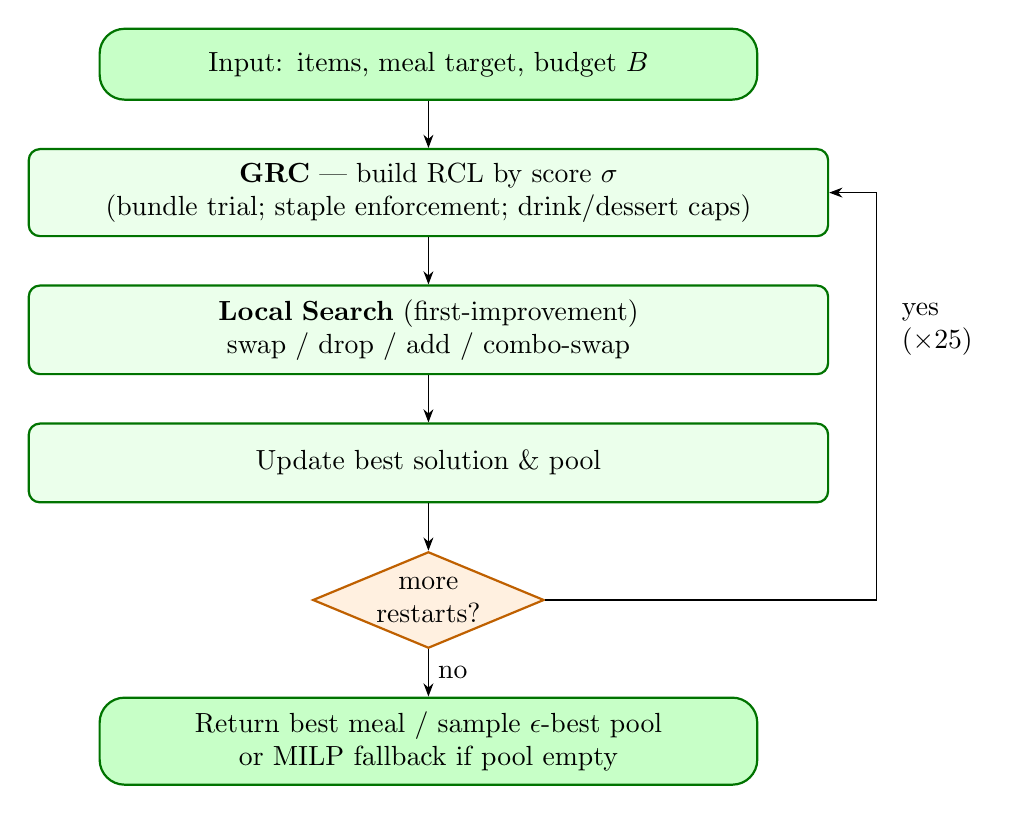
\begin{tikzpicture}[
  font=\normalsize, >=Stealth, node distance=6mm,
  box/.style={rectangle, rounded corners, draw=green!45!black, thick,
              fill=green!8, align=center, inner sep=5pt, text width=98mm, minimum height=10mm},
  term/.style={rectangle, rounded corners=9pt, draw=green!45!black, thick,
               fill=green!22, align=center, inner sep=5pt, text width=80mm, minimum height=9mm},
  dec/.style={diamond, aspect=2.4, draw=orange!75!black, thick, fill=orange!12,
              align=center, inner sep=1pt}]
  \node[term] (in) {Input: items, meal target, budget $B$};
  \node[box, below=of in] (grc) {\textbf{GRC} --- build RCL by score $\sigma$\\(bundle trial; staple enforcement; drink/dessert caps)};
  \node[box, below=of grc] (ls) {\textbf{Local Search} (first-improvement)\\swap / drop / add / combo-swap};
  \node[box, below=of ls] (up) {Update best solution \& pool};
  \node[dec, below=of up] (dec) {more\\restarts?};
  \node[term, below=of dec] (out) {Return best meal / sample $\epsilon$-best pool\\or MILP fallback if pool empty};
  \draw[->] (in) -- (grc);
  \draw[->] (grc) -- (ls);
  \draw[->] (ls) -- (up);
  \draw[->] (up) -- (dec);
  \draw[->] (dec) -- node[right]{no} (out);
  \draw[->] (dec.east) -| ([xshift=6mm]grc.east) |- (grc.east);
  \node[anchor=west, align=left] at ([xshift=8mm]ls.east) {yes\\($\times25$)};
\end{tikzpicture}}
\caption{Overall GRASP-LS workflow. Each restart builds a structurally feasible solution, improves it by local search, and updates the solution pool. Deployment samples from the $\epsilon$-optimal pool and falls back to MILP when needed.}
\label{fig:flow}
\end{figure}

\begin{algorithm}[H]
\caption{GRASP-LS for the Convenience Store Meal Recommendation Problem}
\label{alg:grasp}
\begin{algorithmic}[1]
\Require Instance $\mathcal{I}=(I,K,S)$; constraints $\mathcal{M}$; weights $w$; budget $B$; restarts $K_{\text{restart}}$; window $\epsilon$
\State $\mathcal{P}_{\mathrm{feas}}\gets\emptyset$; $s^* \gets \emptyset$; $z^* \gets +\infty$
\For{$r = 1$ \textbf{to} $K_{\text{restart}}$}
  \State $\alpha_{\text{rcl}} \sim \mathcal{U}(0.10, 0.40)$
  \State $s \gets \textsc{GreedyRandomConstruct}(\mathcal{I},\mathcal{M},w,B,\alpha_{\text{rcl}})$
  \Comment{bundle trial, staple enforcement, and structured filtering}
  \State $s \gets \textsc{LocalSearch}(s,\mathcal{I},\mathcal{M},w,B)$
  \Comment{1-1 swap / 1-0 drop / 0-1 add / combo-swap, first improvement}
  \State $z \gets \textsc{Evaluate}(s)$
  \If{$s$ is hard-feasible}
      \State Add $(s,z)$ to $\mathcal{P}_{\mathrm{feas}}$
      \If{$z < z^*$} $\;s^* \gets s$; $z^* \gets z$ \EndIf
  \EndIf
\EndFor
\If{$\mathcal{P}_{\mathrm{feas}}\ne\emptyset$}
    \State \Return best solution or sample from $\{s:z(s)\le z^*+\epsilon\}$
\Else
    \State Solve the MILP with Gurobi; return its solution if feasible, otherwise report infeasibility and suggest relaxing budget or nutrition constraints
\EndIf
\end{algorithmic}
\end{algorithm}

\paragraph{Time complexity.}At each step, GRC inspects $O(|I|)$ candidates and computes their marginal contributions. It selects at most $N^{\max}_m$ items, so its complexity is $O(N^{\max}_m\cdot |I|)$. In each local-search round, the 1-1 swap neighborhood costs approximately $O(N^{\max}_m\cdot |I|)$. In the worst case, every round improves the solution and triggers another round. In practice, LS converges within $T\le 10$ rounds, giving total runtime $O(K_{\text{restart}}\cdot T\cdot N^{\max}_m\cdot |I|)$.

\begin{algorithm}[H]
\caption{Greedy Randomized Construction (GRC) sub-procedure}
\label{alg:grc}
\begin{algorithmic}[1]
\Require Instance, single-meal constraints, RCL parameter $\alpha_{\text{rcl}}$
\State $s \gets \emptyset$
\If{$\text{Rand}()<0.6$}
    \State Build an RCL of bundles that satisfy budget, calorie, no-overlap, and meal-role caps
    \State Randomly add one bundle $k^*$ only if it contains at most one staple and can help satisfy the required meal structure
\EndIf
\If{regular meal and $s$ contains no staple}
    \State Build a staple-only RCL from feasible uncovered products and randomly add one staple to $s$
\EndIf
\While{$|s|<N^{\max}_m$}
    \State Filter uncovered candidates $C$ that preserve budget, calorie upper bound, at most one drink, at most one dessert, exactly one staple, and no bundle/single overlap
    \If{$C=\emptyset$} \textbf{break} \EndIf
    \If{$\sum cal_i \ge \text{Cal}^{\min}_m$ and $|s|\ge 2$}
        \State Try the top-3 candidates; add a candidate only if it improves the objective; otherwise \textbf{break}
    \Else
        \State Build an $\alpha_{\text{rcl}}$-RCL by $\sigma$ and randomly add one candidate to $s$
    \EndIf
\EndWhile
\State \Return $s$
\end{algorithmic}
\end{algorithm}

\begin{algorithm}[H]
\caption{Local Search (1-1 swap / 1-0 drop / 0-1 add / combo-swap)}
\label{alg:ls}
\begin{algorithmic}[1]
\Require Solution $s$, maximum number of rounds $T_{\max}$
\For{$t = 1$ \textbf{to} $T_{\max}$}
  \State $\text{improved} \gets \texttt{false}$
  \ForAll{$p \in s$, $p'\notin s$}
    \If{replacing $p$ with $p'$ is feasible and lowers the objective}
      \State $s \gets s\setminus\{p\}\cup\{p'\}$; $\text{improved}\gets\texttt{true}$; \textbf{break to outer}
    \EndIf
  \EndFor
  \If{\textbf{not} improved} Try 1-0 drop, 0-1 add, and combo-swap \EndIf
  \If{no move improves the solution in this round} \textbf{break} \EndIf
\EndFor
\State \Return $s$
\end{algorithmic}
\end{algorithm}

\paragraph{Diversity-aware deployment: $\epsilon$-optimal sampling and fallback solving.}\label{par:eps}
If the system always returns the unique best solution, consecutive queries may produce almost identical meals. MILP is deterministic, and diversity would rely only on historical penalties. This study therefore formalizes diversity as uniform sampling from an $\epsilon$-optimal solution set $\mathcal{S}_\epsilon=\{s : z(s)\le z^*+\epsilon\}$. For each query, the system randomly samples one solution whose objective value is within $\epsilon$ of the best solution. The parameter $\epsilon$ directly controls the trade-off between diversity and optimality, as quantified in \S\ref{sec:div}. In deployment, GRASP-LS with $\epsilon=8$ is used to provide diversified recommendations. If GRASP-LS fails to find a feasible solution under an extremely tight budget, the system falls back to exact MILP solving to ensure that a recommendation is returned whenever a feasible solution exists.

\section{Data Collection and Generation}\label{sec:data}
\paragraph{Real-world data scraping.}Real-world data were collected in three stages:
\begin{enumerate}
\item \textbf{Nutrition labels.} We collected official nutrition labels for \textbf{581 FamilyMart products} from the food-safety traceability API (\url{foodsafety.family.com.tw/Web_FFD_2022/ws/QueryFsProductListByFilter} and \texttt{QueryFsProductByItem}), covering 22 categories. Calories, protein, fat, carbohydrates, sugar, and sodium come from official package-level labels, with serving counts used to convert values to package totals. The scraper is \texttt{src/scrape\_familymart.py}.
\item \textbf{Prices.} Because the food-safety API lacks prices, prices were assigned before or during curation. We parsed FamilyMart's fresh-food promotion page (\url{nevent.family.com.tw/freshfood/}) and matched \textbf{124 raw fresh-food products} to real in-store tiered prices (NT\$49/59/69/79/99/109) using n-gram fuzzy matching. The remaining raw non-fresh-food products used category-calibrated estimates, because no public single-item in-store price API is available. The e-commerce catalog (\texttt{fts-api.91app.com}) is unsuitable because 78\% of items are box or multi-pack products, so direct use would distort single-meal prices. We therefore assigned market-calibrated estimates by category, such as NT\$28 for dairy or bottled soy milk, NT\$20 per oden item, and NT\$59 for sous-vide chicken breast, with volume adjustments for beverages. Accordingly, we explicitly label the data sources: fresh foods use real tiered prices, while other products use reasonable market-calibrated estimates. The scripts are \texttt{src/scrape\_freshfood\_prices.py} and \texttt{src/curate\_prices.py}.
\item \textbf{Serving normalization, family-size filtering, and role labeling.} Multi-serving SKUs were normalized to a per-serving basis, with a NT\$18 per-serving price floor to avoid unrealistically cheap package averages. Family-size products with at least three servings were removed. After serving normalization, family-size filtering, and role-label curation, the final optimization dataset contains \textbf{488 usable single-meal products}. Because keyword-based \texttt{is\_main}/\texttt{is\_protein} flags were noisy, we reassigned meal roles using official categories and reclassified sweet breads with sugar $\ge 10$ g as desserts. This better reflects realistic single-meal consumption. The processing logic is in \texttt{src/data\_loader.py}.
\end{enumerate}

\paragraph{Promotional bundles.}We generated 55 scenario-based promotional bundles of three types: staple + drink, staple + side, and staple + side + drink, with 17\%--20\% discounts. These are synthetic bundle instances because FamilyMart promotion pages change frequently and do not expose a stable public bundle API. The bundle patterns and discount ranges match common convenience-store promotion formats, so real nutrition and price data are combined with controlled promotional scenarios.

\paragraph{Real-world user profiles.}To demonstrate how recommendations differ across user conditions, we designed six representative profiles based on realistic demographic settings, gender, health goal, and activity level. They are scenario-based real-world instances rather than private user logs. Each profile was paired with three meal scenarios, producing 18 real-world instances (Table \ref{tab:real}).

\paragraph{Random instances.}To evaluate scalability, random instances used six sizes from 30 to 300 products, with bundle counts from 8 to 90. Five random seeds were used for each size, yielding 30 random instances. Product attributes were generated as follows: $cal\sim \mathcal{U}(180,650)$ for staple items or $\mathcal{U}(15,320)$ for non-staples, $pro\sim \mathcal{U}(5,30)$ for protein-containing items or $\mathcal{U}(0,10)$ otherwise, and $sod\sim \mathcal{U}(0,1400)$. Bundle sizes were in $\{2,3\}$, and discount rates were sampled from $\mathcal{U}(0.80,0.92)$ of the original price.

\paragraph{Stress-test scenarios (factorial scenario design).}To test robustness beyond scale, we used a $2\times2$ design crossing budget (tight $B=90$ vs. loose $B=220$) and protein target (muscle-gain high vs. maintenance relaxed). Crossing these with three sizes and four seeds produced $4\times3\times4=48$ instances, solved by MILP and GRASP-LS using \texttt{src/run\_extra\_experiments.py} (\S\ref{sec:stress}).

\section{Performance Evaluation}\label{sec:exp}
This section compares three solution methods: (i) \textbf{Gurobi MILP}, the exact benchmark for optimality or bounds; (ii) \textbf{GRASP-LS}, the self-proposed heuristic designed for deployability; and (iii) \textbf{Basic Greedy}, a deliberately simple protein-to-price-ratio heuristic benchmark. Basic Greedy is not intended to be competitive after meal-structure constraints are introduced; it is included to show why a one-dimensional shopping rule is inadequate. A stronger repaired greedy baseline is discussed as a limitation, but it is not reported numerically because it was not part of the implemented experimental pipeline. The weights are set to $\alpha=1, \beta=0.5, \gamma=2, \gamma_{\text{cat}}=8, \lambda_P=6, \lambda^\pm_F = 2/3, \lambda^\pm_C = 1/1.5, \lambda_{\text{Sug}}=4, \lambda_{\text{Sod}}=0.15$. All benchmark tables are solved with empty history, so diversity penalties do not affect the optimal values. Real-world instances demonstrate practicality, while random and stress-test instances test scalability and robustness within the tested settings.

\subsection{Real-world Instances}
Table \ref{tab:real} reports the results for six real-world users across three scenarios. MILP obtained the global optimum for all 18 instances. GRASP-LS also achieved \textbf{100\% hard-feasibility}, with an average optimality gap of \textbf{7.1\%}; 12 out of 18 instances had zero gap. Importantly, all nonzero gaps occurred in the regular-meal scenario. After the exactly-one-staple and meal-structure constraints (C10--C11) were introduced, the feasible region for regular meals became narrower, and the 1-1 swap neighborhood in GRASP-LS occasionally became trapped in a local optimum, with the worst case being U5 female-maintenance-regular at 40.5\%. By contrast, light meals and late-night meals all had zero gap. \textbf{Basic Greedy was 0\% feasible under the new structure and hard sodium cap}: it greedily selects small high-protein products according to the protein-to-price ratio, which typically leads to missing a staple item (violating C11) and exceeding the $1.5\times$ sodium cap (violating C8b). This highlights the difficulty of handling multiple structural constraints with a single sorting criterion (Figure \ref{fig:feas}).

\begin{table}[htbp]
\centering\small
\caption{Results for the 18 real-world instances. Gap is $(z_{\text{GRASP-LS}}-z_{\text{MILP}})/|z_{\text{MILP}}|$. MILP returns global optima; GRASP-LS is 100\% hard-feasible with a 7.1\% average gap; Basic Greedy is 0\% feasible.}
\label{tab:real}
\begin{tabular*}{\textwidth}{@{\extracolsep{\fill}}lrrrrrccc@{}}
\toprule
 & & & & & & \multicolumn{3}{c}{Feasible (Y/N)} \\
\cmidrule(lr){7-9}
Instance & Cal range & $P^{\min}$ & MILP obj & GRASP-LS obj & Gap (\%) & MILP & GRASP-LS & Greedy \\
\midrule
U1\_male\_cut-latenight & 106--318 & 11.2 & 27.98 & 27.98 & 0.0 & Y & Y & N \\
U1\_male\_cut-light & 318--529 & 22.4 & 35.80 & 35.80 & 0.0 & Y & Y & N \\
U1\_male\_cut-regular & 635--953 & 44.8 & 87.20 & 119.48 & 37.0 & Y & Y & N \\
U2\_male\_bulk-latenight & 166--497 & 13.5 & 40.60 & 40.60 & 0.0 & Y & Y & N \\
U2\_male\_bulk-light & 497--829 & 27.0 & 68.09 & 68.09 & 0.0 & Y & Y & N \\
U2\_male\_bulk-regular & 994--1491 & 54.0 & 163.53 & 173.55 & 6.1 & Y & Y & N \\
U3\_male\_maintain-latenight & 98--293 & 7.7 & 29.55 & 29.55 & 0.0 & Y & Y & N \\
U3\_male\_maintain-light & 293--489 & 15.4 & 36.21 & 36.21 & 0.0 & Y & Y & N \\
U3\_male\_maintain-regular & 587--880 & 30.8 & 74.04 & 74.85 & 1.1 & Y & Y & N \\
U4\_female\_cut-latenight & 73--220 & 8.3 & 32.91 & 32.91 & 0.0 & Y & Y & N \\
U4\_female\_cut-light & 220--366 & 16.6 & 41.17 & 41.17 & 0.0 & Y & Y & N \\
U4\_female\_cut-regular & 439--658 & 33.3 & 67.74 & 75.05 & 10.8 & Y & Y & N \\
U5\_female\_maint-latenight & 77--232 & 6.1 & 29.62 & 29.62 & 0.0 & Y & Y & N \\
U5\_female\_maint-light & 232--387 & 12.1 & 35.80 & 35.80 & 0.0 & Y & Y & N \\
U5\_female\_maint-regular & 464--697 & 24.2 & 63.20 & 88.82 & 40.5 & Y & Y & N \\
U6\_female\_bulk-latenight & 132--395 & 10.4 & 35.75 & 35.75 & 0.0 & Y & Y & N \\
U6\_female\_bulk-light & 395--659 & 20.9 & 57.55 & 57.55 & 0.0 & Y & Y & N \\
U6\_female\_bulk-regular & 791--1186 & 41.8 & 106.60 & 140.65 & 31.9 & Y & Y & N \\
\bottomrule
\end{tabular*}
\end{table}

Figure \ref{fig:break} uses U1 (male, fat loss, regular meal) as an example to compare the nutritional and cost outcomes of the three methods. MILP and GRASP-LS both produce structurally complete meals that satisfy all relevant targets. Greedy, because it only considers the protein-to-price ratio, misses the staple requirement and exceeds the hard sodium cap, making the solution hard-infeasible.

\begin{figure}[htbp]
\centering
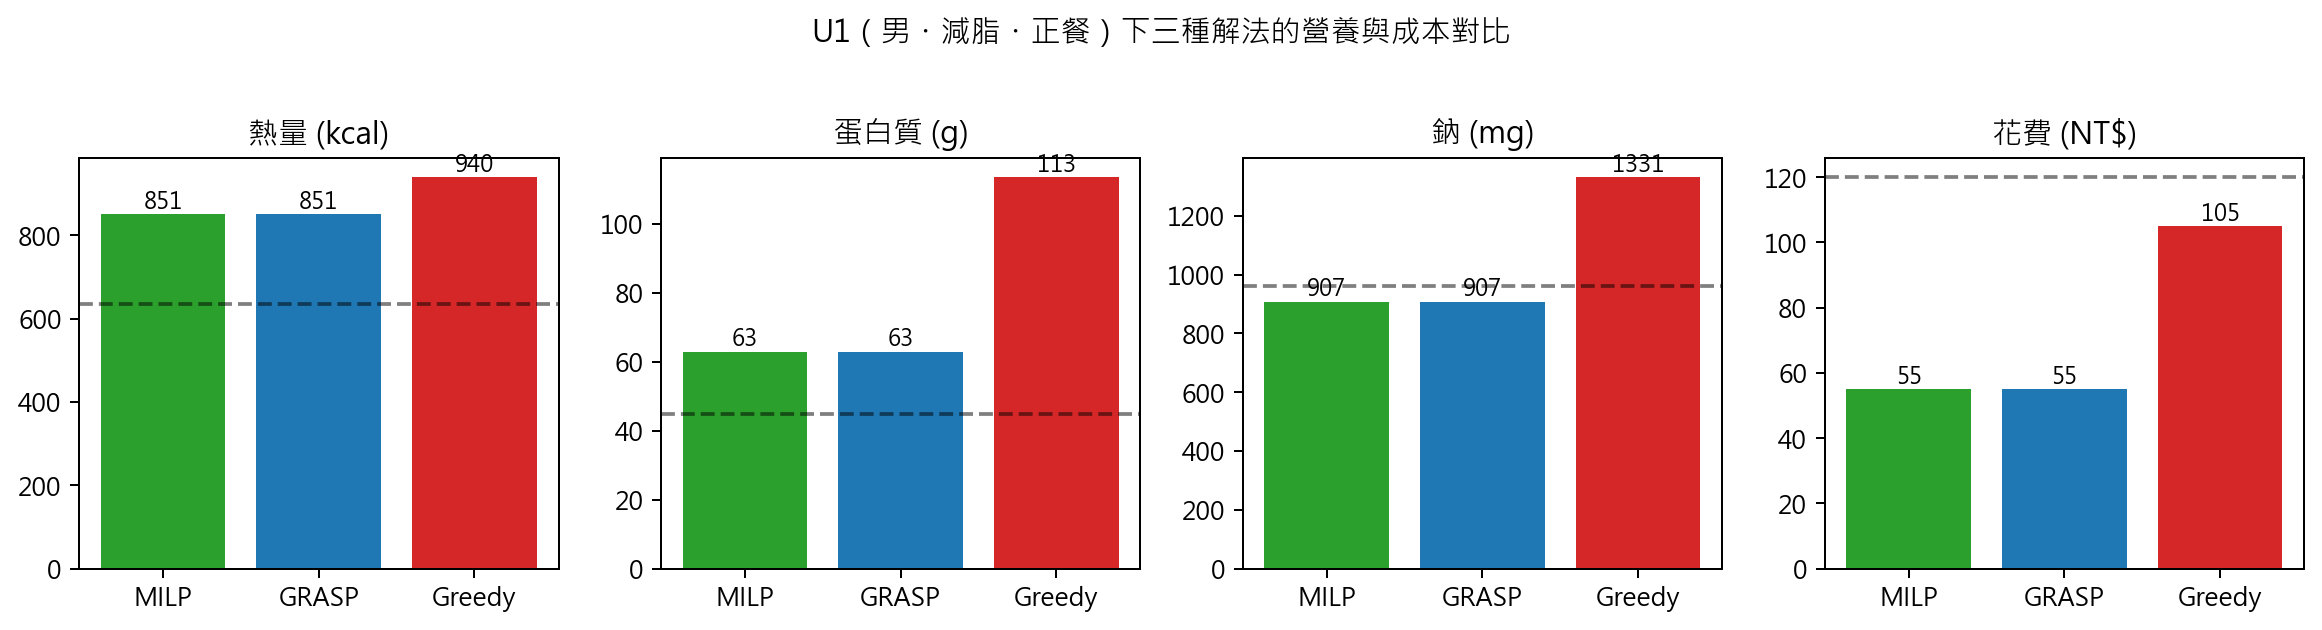
\includegraphics[width=0.95\textwidth]{../results/figs/fig_real_breakdown.png}
\caption{Calories, protein, sodium, and cost for U1 male-fat-loss-regular. MILP and GRASP-LS satisfy all requirements, while Greedy lacks a staple item and exceeds the hard sodium cap.}
\label{fig:break}
\end{figure}

\begin{figure}[htbp]
\centering
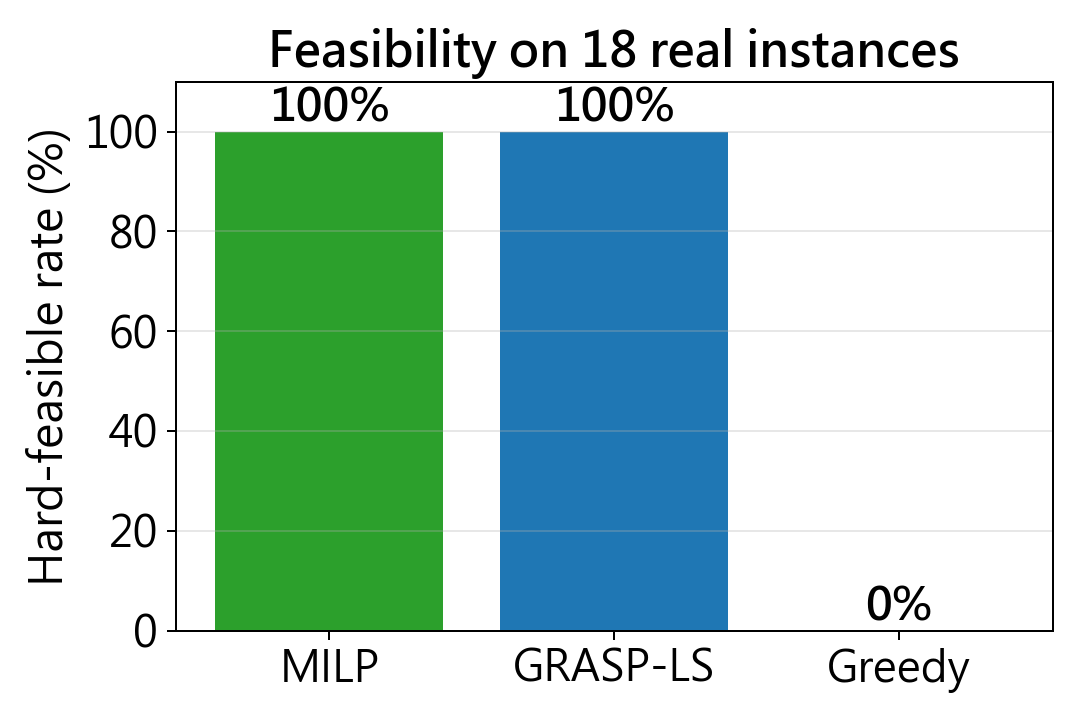
\includegraphics[width=0.58\textwidth]{../results/figs/fig_feasibility.png}
\caption{Hard-feasibility rates across 18 real-world instances.}\label{fig:feas}
\end{figure}

\FloatBarrier
\subsection{Random Instances and Scalability}
The results of the 30 random instances are reported in Table \ref{tab:rand} and Figures \ref{fig:gap}--\ref{fig:rt}.
MILP found the optimum at every size. GRASP-LS achieved an aligned average optimality gap of \textbf{4.9\%} over the \textbf{28} instances where both MILP and GRASP-LS were feasible, and its hard-feasibility rate was 93\% (28/30). The two cases where GRASP-LS did not find a feasible solution occurred in tight-budget instances with $|I|=30$ and $|I|=50$. Under the structural constraints, construction may occasionally fail to assemble a low-budget meal that contains exactly one staple, at least one protein source, and enough calories. In deployment, these cases are handled by the MILP fallback.

To avoid comparing objectives averaged over different feasibility subsets, Table \ref{tab:rand} reports MILP objective, GRASP-LS feasibility, and aligned GRASP-LS gaps rather than size-level GRASP-LS objective averages. By contrast, after adding the meal-structure constraints (C10--C11) and the hard sodium cap (C8b), Basic Greedy almost completely fails, with \textbf{0\% feasibility} in most sizes. This confirms the need for multi-constraint optimization.

Figure \ref{fig:rt} shows how runtime grows with the number of products. MILP increased from 6 ms at $|I|=30$ to 227 ms at $|I|=300$. GRASP-LS increased from 14 ms to approximately 4.2 seconds. Greedy remained below the millisecond level. Although Gurobi was faster at the tested scale, GRASP-LS provides practical advantages: it avoids commercial-license dependence, can run in environments where a solver is unavailable, naturally generates multiple near-optimal candidates for $\epsilon$-diversity, and has an anytime property. In deployment, Gurobi is therefore treated as the quality benchmark and fallback solver, while GRASP-LS is the self-proposed deployable recommendation algorithm.

\begin{table}[htbp]
\centering\normalsize
\caption{Average performance across random-instance sizes, with five seeds per size. MILP objective is averaged over all five runs. Times are in seconds. GRASP-LS gap is the aligned average $(z_{\text{GRASP-LS}}-z_{\text{MILP}})/|z_{\text{MILP}}|\times100\%$ over instances where both methods are feasible.}
\label{tab:rand}
\begin{tabular*}{\textwidth}{@{\extracolsep{\fill}}rrrrrrrr@{}}
\toprule
$|I|$ & $|K|$ & MILP obj & MILP time & GRASP-LS feas & GRASP-LS gap & GRASP-LS time & Greedy feas \\
\midrule
30 & 8  & 143.5 & 0.006 & 4/5 & 3.1  & 0.014 & 0/5 \\
50 & 15 & 111.4 & 0.023 & 4/5 & 4.5  & 0.046 & 1/5 \\
80 & 25 & 74.3  & 0.020 & 5/5 & 0.0  & 0.104 & 0/5 \\
120& 35 & 58.6  & 0.075 & 5/5 & 5.0  & 0.576 & 0/5 \\
200& 60 & 50.3  & 0.133 & 5/5 & 11.6 & 2.044 & 0/5 \\
300& 90 & 42.1  & 0.227 & 5/5 & 4.5  & 4.156 & 0/5 \\
\bottomrule
\end{tabular*}
\end{table}
\begin{figure}[htbp]
\centering
\begin{minipage}{0.48\textwidth}\centering
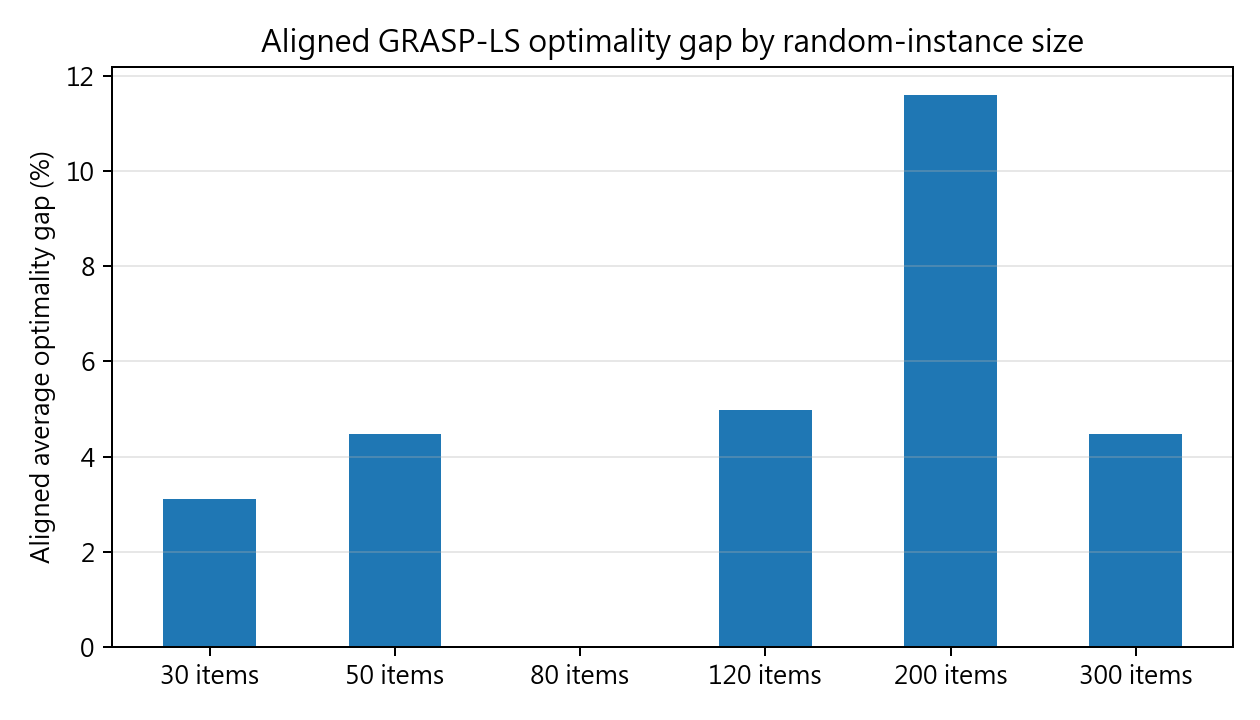
\includegraphics[width=\textwidth]{../results/figs/fig_gap_by_size.png}
\caption{Aligned average GRASP-LS optimality gap by random-instance size, computed only over instances where both MILP and GRASP-LS are feasible.}
\label{fig:gap}
\end{minipage}\hfill
\begin{minipage}{0.48\textwidth}\centering
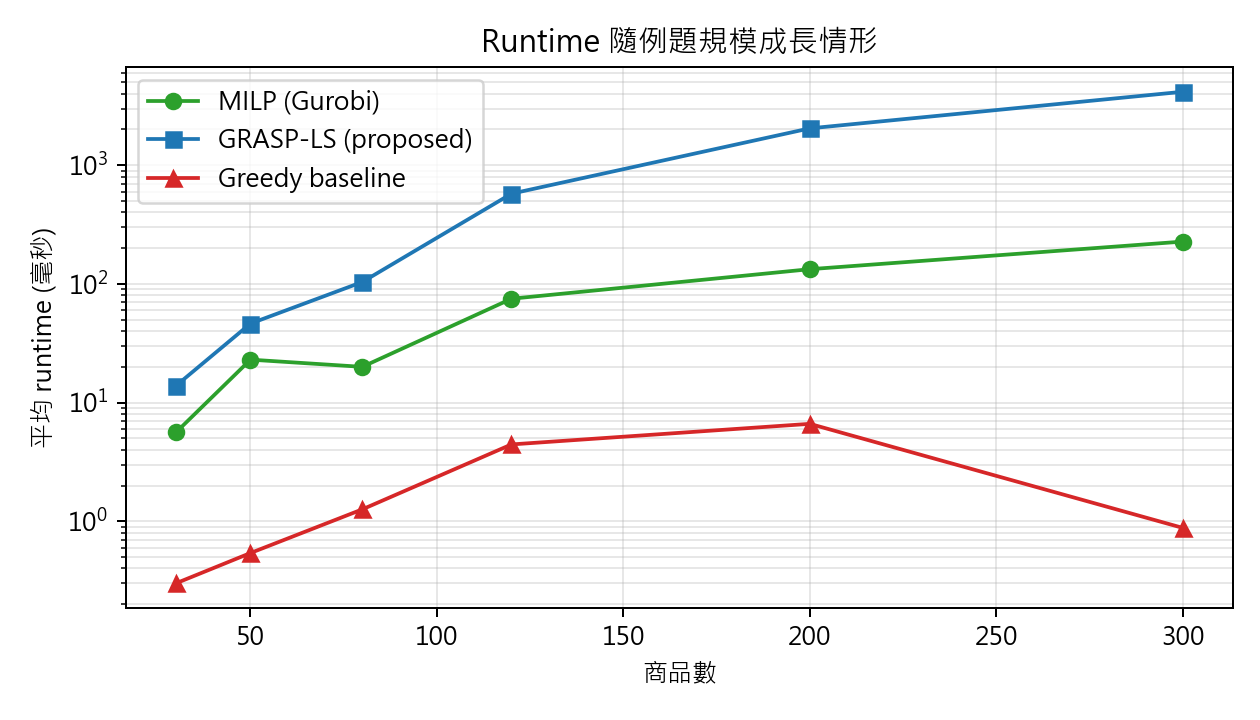
\includegraphics[width=\textwidth]{../results/figs/fig_runtime.png}
\caption{Effect of random-instance size on solution time (log scale).}\label{fig:rt}
\end{minipage}
\end{figure}
\FloatBarrier

\subsection{Stress-test Scenarios}\label{sec:stress}
Table \ref{tab:stress} summarizes the $2\times2$ stress-test scenarios, where budget and protein target are crossed and each cell contains 12 instances. MILP was feasible in all 48 instances. GRASP-LS found feasible solutions in \textbf{46/48} instances. Both failures occurred under the tight-budget condition, one with a high protein target and one with a relaxed protein target. In our stress-test design, the high protein target appears to be a stronger driver of the optimality gap than the tight budget alone. Under the muscle-gain goal, the gaps were 7.4\% for tight budgets and 4.1\% for loose budgets; under the maintenance goal, the gaps were only 1.2\% and 1.4\%. Tight-budget scenarios were faster because the feasible region was smaller (about 1.1--1.2 seconds for GRASP-LS, compared with 2.7--2.9 seconds under loose budgets). Within these tested settings, GRASP-LS kept the average gap no greater than 7.4\% and solved the instances within seconds.
\begin{table}[htbp]
\centering\normalsize
\caption{$2\times2$ stress-test scenarios, with 12 instances per cell: MILP/GRASP-LS feasibility, average GRASP-LS optimality gap, and average solution time.}
\label{tab:stress}
\begin{tabular}{lcccc}
\toprule
Scenario (budget $\times$ protein) & MILP feas & GRASP-LS feas & avg gap & GRASP-LS time \\
\midrule
Tight $\times$ high protein & 12/12 & 11/12 & 7.35\% & 1.10 s \\
Tight $\times$ relaxed      & 12/12 & 11/12 & 1.22\% & 1.24 s \\
Loose $\times$ high protein & 12/12 & 12/12 & 4.12\% & 2.85 s \\
Loose $\times$ relaxed      & 12/12 & 12/12 & 1.36\% & 2.72 s \\
\bottomrule
\end{tabular}
\end{table}

\subsection{Comparison with an Uninformed Shopper}\label{sec:human}
To estimate value relative to unaided shopping, we randomly sampled 2--4 products within each user's budget for 4000 trials over the 488 real products (\texttt{src/run\_extra\_experiments.py}). Table \ref{tab:human} shows that random selection satisfies all meal constraints only about \textbf{4\%} of the time; the protein lower bound is met about \textbf{6\%} of the time, while sodium is acceptable about 63\% of the time. GRASP-LS achieves \textbf{100\%} target satisfaction. Its average cost (about NT\$109) is comparable to blind selection (about NT\$99), so the improvement comes from better composition rather than simply buying less.
\begin{table}[htbp]
\centering\normalsize
\caption{Uninformed shopper baseline vs. model. Each user is simulated with 4000 random samples. Percentages indicate how often blind selection satisfies each constraint. Model cost is the cost of the GRASP-LS compliant meal.}
\label{tab:human}
\begin{tabular}{lccccc}
\toprule
User & All targets & Protein target & Sodium target & Blind avg. cost & Model cost \\
\midrule
U1 male-fat loss & 5.2\% & 1.6\%  & 59.5\% & NT\$103.7 & NT\$108 \\
U2 male-bulk     & 0.4\% & 1.3\%  & 47.7\% & NT\$121.6 & NT\$149 \\
U3 male-maintain & 3.2\% & 7.1\%  & 71.7\% & NT\$89.5  & NT\$93  \\
U4 female-fat loss & 9.8\% & 5.0\%  & 70.1\% & NT\$89.7  & NT\$94  \\
U5 female-maintain & 3.7\% & 14.6\% & 74.2\% & NT\$80.6  & NT\$85  \\
U6 female-bulk     & 1.9\% & 4.0\%  & 53.2\% & NT\$110.9 & NT\$124 \\
\bottomrule
\end{tabular}
\end{table}

\subsection{Sensitivity Analysis}
Figure \ref{fig:beta} shows the cost-protein trade-off when the budget is relaxed to NT\$220 and the protein weight $\beta$ is varied. When $\beta\le 1$, the model selects an NT\$109.5 combination that just satisfies the protein lower bound (45.6 g). Once $\beta\ge 2$, the marginal benefit of protein exceeds the cost threshold of more expensive high-protein products, so the model changes the recommendation. Protein increases sharply to 92.8 g, and spending rises to NT\$177. At $\beta=8$, the meal reaches 119.5 g of protein and costs NT\$201.5. This stepwise jump reflects the discrete nature of MILP decisions. Figure \ref{fig:gamma} shows the diversity effect of tiered memory. After the optimal solution under $\gamma=0$ is injected into recent history, all four items reappear when $\gamma=0$. Once $\gamma\ge 1$, the tiered penalty causes the model to replace all recommended items, reducing the repetition count to zero. Because the substitutes are similarly inexpensive, total cost even decreases from NT\$109.5 to NT\$103. This indicates that historical penalties can substantially improve diversity with almost no cost sacrifice.
\begin{figure}[htbp]
\centering
\begin{minipage}{0.48\textwidth}\centering
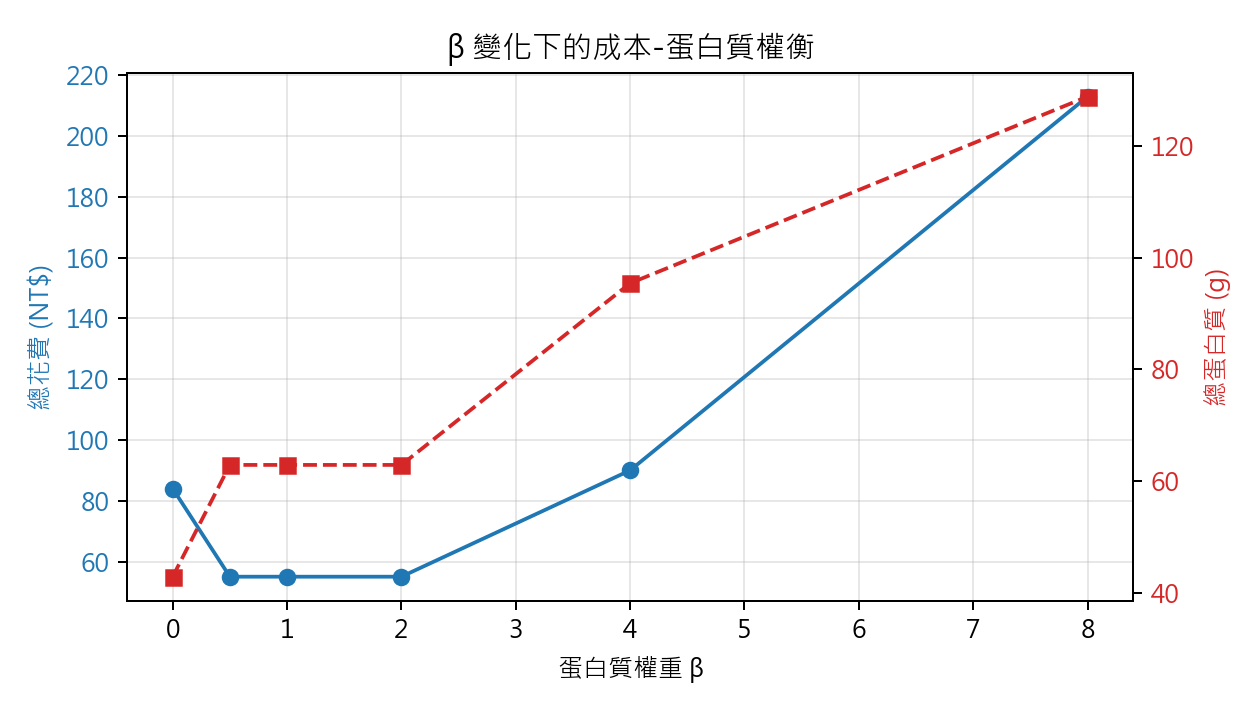
\includegraphics[width=\textwidth]{../results/figs/fig_beta_tradeoff.png}
\caption{Cost-protein trade-off under different values of $\beta$.}\label{fig:beta}
\end{minipage}\hfill
\begin{minipage}{0.48\textwidth}\centering
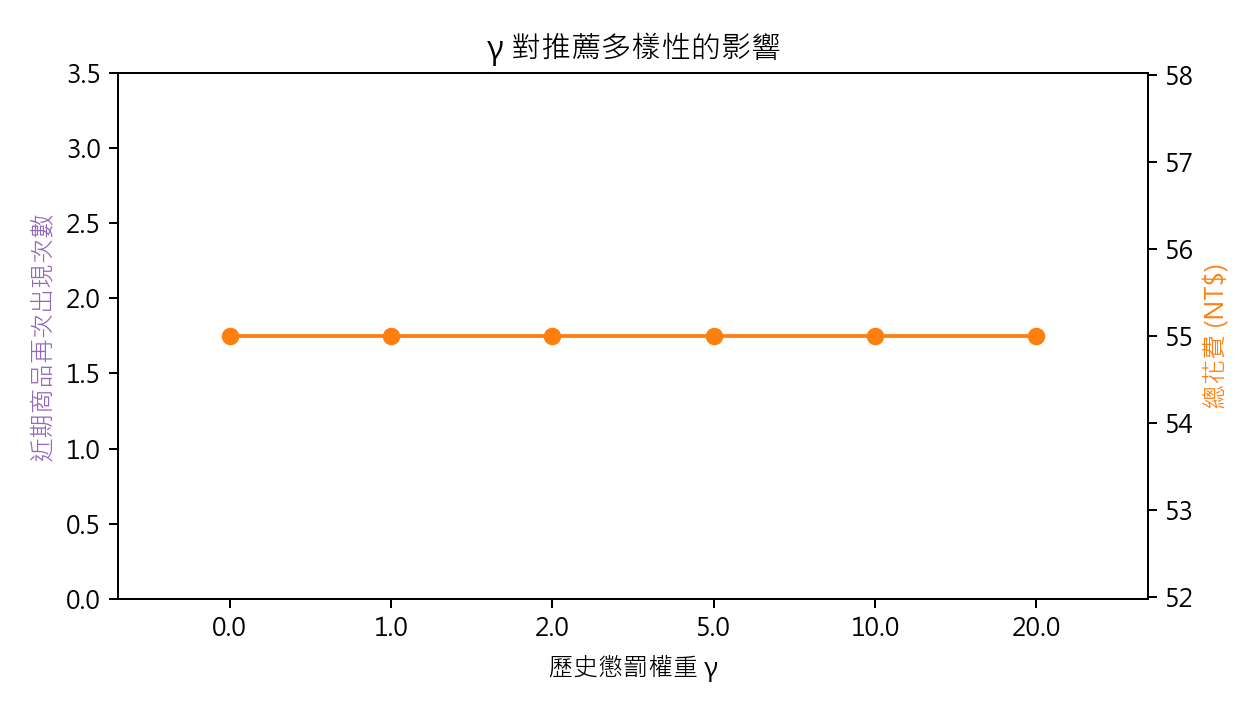
\includegraphics[width=\textwidth]{../results/figs/fig_gamma_diversity.png}
\caption{Decline in recently repeated items as $\gamma$ increases.}\label{fig:gamma}
\end{minipage}
\end{figure}

\subsection{The Price of Diversity}\label{sec:div}
Using the Gurobi solution pool (\texttt{PoolSearchMode=2}), we enumerate $\mathcal{S}_\epsilon=\{s:z(s)\le z^*+\epsilon\}$ to quantify diversity cost. For a male-maintenance-regular user with a cheapest compliant meal of NT\$93, Figure \ref{fig:div} shows that $\epsilon=0$ yields one meal; $\epsilon=8$ yields \textbf{12} distinct compliant meals with only NT\$6.7 average extra cost. At $\epsilon=16$ and $32$, the counts rise to \textbf{48} and \textbf{641}. Thus, near-optimal diversity is inexpensive. Deployment samples from this set with $\epsilon=8$, approximated by GRASP-LS and tiered memory.
\begin{figure}[htbp]
\centering
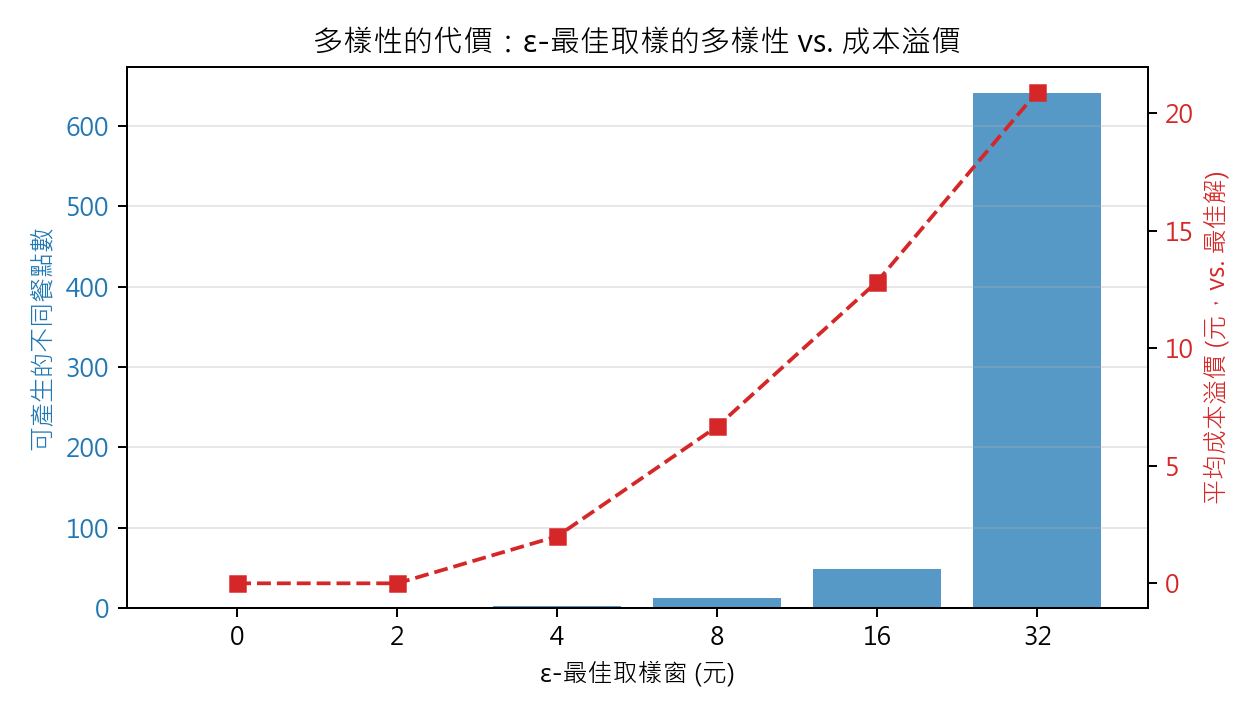
\includegraphics[width=0.62\textwidth]{../results/figs/fig_price_of_diversity.png}
\caption{The price of diversity. As the $\epsilon$-optimal sampling window is relaxed, the number of distinct compliant meals increases from 1 to 641 (blue bars), while the average cost premium (red line) rises only gradually to about NT\$21. Near the optimum, diversity is inexpensive.}
\label{fig:div}
\end{figure}

\subsection{Executable Recommendations}
In U1 male-fat-loss-regular (70 kg, TDEE 2118 kcal, budget NT\$120), the MILP solution is pineapple bun + honey pork jerky + unsweetened thick soy milk + mixed fruit gummies, costing NT\$110 with 693 kcal, 45.6 g protein, and 667 mg sodium. It satisfies the staple, protein-source, calorie, protein, and sodium requirements. Greedy selects chicken thigh steak + pig-ear strips + soy milk (NT\$118, 91 g protein), but lacks a staple and reaches 2168 mg sodium, so it is unacceptable. The model's value lies not merely in reducing cost; it reliably produces meals that are structurally reasonable, nutritionally compliant, and diverse over repeated use.

\subsection{Interactive Web Application}
To validate usability, we implement a Flask web app (\texttt{webapp/app.py}). Users enter physiological information and meal context; the backend calls GRASP-LS with $\epsilon$-optimal sampling by default, or Gurobi MILP, and returns recommendations. Cookies maintain a tiered ``taste memory'' queue, and sliders adjust $\alpha,\beta,\gamma$. Figure \ref{fig:webapp} shows the interface.
\begin{figure}[htbp]
\centering
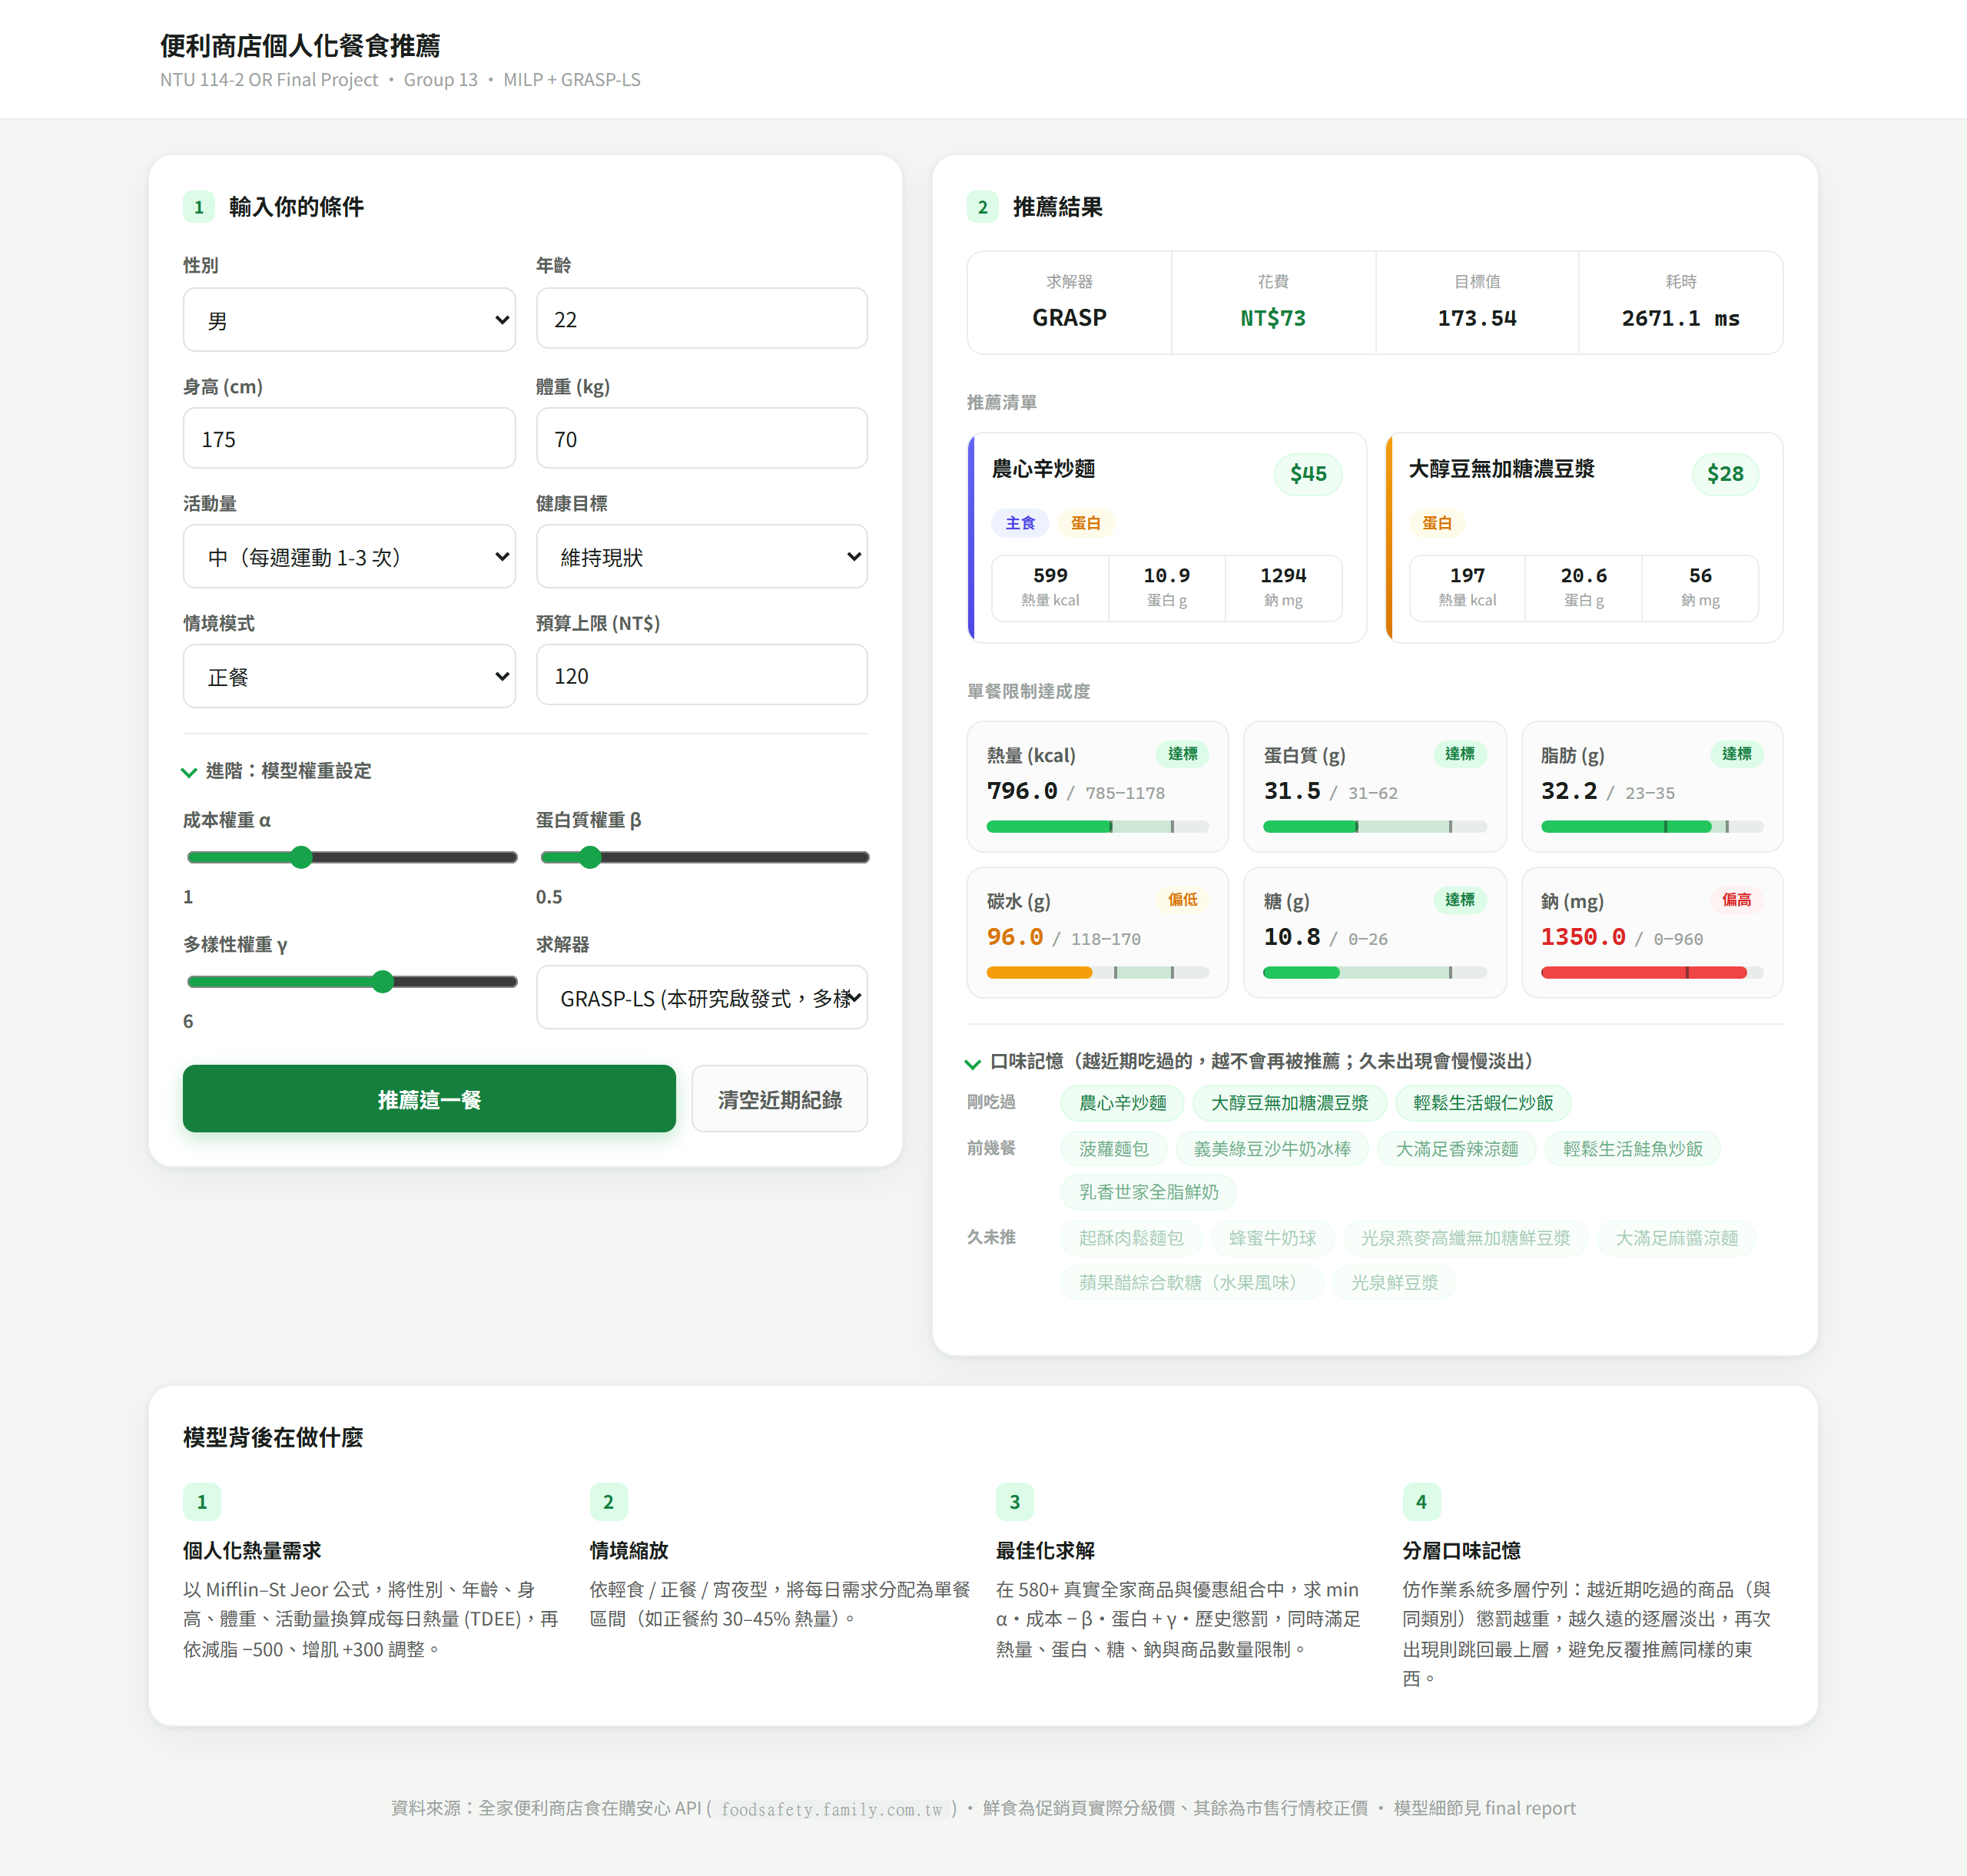
\includegraphics[width=0.95\textwidth]{../results/figs/webapp_result.png}
\caption{Interactive web application with the advanced weight panel and tiered taste-memory panel expanded. For a male, 22-year-old, 175 cm, 70 kg, moderate-activity user with maintenance goal, regular meal, and NT\$120 budget, GRASP-LS returns a structurally complete meal and nutrition-target status. The backend uses the 488-product curated optimization dataset.}
\label{fig:webapp}
\end{figure}
\FloatBarrier

\subsection{Discussion and Limitations}
\paragraph{Why is Basic Greedy 0\% feasible under the new model?}Basic Greedy ranks items only by protein-to-price ratio, so it tends to select cheap, protein-dense items such as chicken and soy milk. It then violates multiple hard constraints: no staple item (C11), mostly side items, and excess sodium from processed high-protein products (C8b). This confirms that realistic meal recommendation is a multi-constraint combinatorial optimization problem, not a single-ratio ranking task.

\paragraph{Baseline limitation.}Because Basic Greedy has no repair phase, its 0\% feasibility should be interpreted as a lower-bound benchmark rather than the strongest possible heuristic baseline. A natural next benchmark is Greedy+Repair: first force one staple and one protein source, then repair calorie, sodium, drink, dessert, and budget violations by local swaps. This would make the comparison stricter, but it would also become close to a simplified version of GRASP-LS. We therefore report Basic Greedy transparently and leave Greedy+Repair as a future benchmark.

\paragraph{Why are GRASP-LS gaps sometimes larger in regular-meal instances?}C10--C11 make the regular-meal feasible region narrower. If construction selects a non-optimal staple and 1-1 swaps cannot reach the optimum in one step, LS may become trapped. The largest regular-meal gaps suggest adding staple-replacement, 2-2 swap, or path-relinking moves in future versions. Increasing $K_{\text{restart}}$ or using MILP fallback can also mitigate this issue.

\paragraph{Meal-structure constraints improve realism.}Without C10--C11 and role labels, earlier versions could produce nutritionally compliant but unrealistic meals, such as dessert as the main item or an entire 1857 ml bottle of soy milk. With official role labels, family-size filtering, and structural constraints, recommendations now resemble practical meals: one staple plus a side and/or drink, with at most one dessert.

\paragraph{Data quality and price estimation.}Nutrition data start from 581 official traceability records and, after serving normalization, family-size filtering, and role curation, yield 488 usable single-meal products for optimization. During price assignment, 124 raw fresh-food items use real tiered prices and the remaining raw non-fresh-food items use category-based market-calibrated estimates, because no public single-item in-store price API exists and the e-commerce catalog mostly contains multi-pack prices. This is the main data limitation. However, under $\pm10\%$ price perturbation, the U1 regular-meal structure remains unchanged, suggesting limited sensitivity to small price errors in this tested case.

\paragraph{Weight selection.}The default weights are $(\alpha, \beta, \gamma)=(1, 0.5, 2)$, and the sensitivity analysis illustrates how these weights affect the solution. In practical deployment, these weights can be exposed through app sliders, allowing users to choose whether they care more about cost or protein. They can also be learned automatically from personal historical feedback.

\section{Conclusions}
This study formulates convenience-store meal recommendation as a mixed-integer linear program with promotional bundles, personalized nutrition constraints, meal-structure constraints, and tiered diversity penalties. Starting from 581 raw FamilyMart nutrition records, price assignment and curation produce a final optimization dataset of 488 usable single-meal products. We develop a self-proposed GRASP-LS heuristic with structure-aware construction, local search, MILP fallback, and $\epsilon$-optimal diversified sampling, then evaluate it on 18 real-world and 30 random instances. The main findings are: (1) MILP obtains global optima within milliseconds to seconds and serves as the benchmark; (2) GRASP-LS achieves 100\% hard-feasibility in real-world instances, with 7.1\% and 4.9\% aligned average gaps for real-world and random instances; (3) after adding meal-structure constraints and the hard sodium cap, the Greedy baseline achieves \textbf{0\% feasibility}; (4) $\beta$ controls the cost-protein trade-off stepwise, while tiered memory removes repetition with almost no price increase; (5) near the optimum, an NT\$8 window yields 12 compliant meals and an NT\$32 window yields 641, showing that diversity is inexpensive in the tested case; and (6) the Flask web application demonstrates deployment potential.

Future work includes a Greedy+Repair benchmark, richer local-search neighborhoods, multi-day recommendation, dynamic inventory information, OCR-based in-store label updates, online learning from clicks and rejections, and integration with delivery apps or other channels such as 7-11 and Hi-Life.

\section*{References}
\small
[1] M. D. Mifflin et al., ``A new predictive equation for resting energy expenditure in healthy individuals,'' \textit{American Journal of Clinical Nutrition}, 1990. [2] T. A. Feo and M. G. C. Resende, ``Greedy randomized adaptive search procedures,'' \textit{Journal of Global Optimization}, 1995. [3] Gurobi Optimization, LLC, \textit{Gurobi Optimizer Reference Manual}, \url{https://www.gurobi.com/documentation/}. [4] FamilyMart, Food Safety Traceability API, \url{foodsafety.family.com.tw/Web_FFD_2022/ws/QueryFsProductListByFilter}, and Fresh Food Promotion Pages, \url{https://nevent.family.com.tw/freshfood/}, accessed 2026.

\end{document}
